\chapter{Minecraft as a MicroPsi 2 World}
The objective of this project is to build and test an interface in between MicroPsi and Minecraft, so that a Minecraft world can be used as a simulation environment for experiments within the MicroPsi framework, which will act as an artificial player. Since there exist open source projects that perform many of the tasks required for this goal, \texttt{Spock}, the Python Minecraft bot framework by Nick Gamberini, and \texttt{Minecraft}, the Python Minecraft clone by Michael Fogleman, have been chosen as a foundation. To make the new simulation environment monitorable, the latter has been used to implement a visualisation of the Minecraft world in the web interface. The following section gives an overview of the implemented modules.

\section{Overview}
The modular architecture of MicroPsi allows it to add new simulation environments (or worlds, as they are called in MicroPsi) fairly easily. To communicate with a MicroPsi node net, a world needs an interface, which is called \emph{world adapter}. The \emph{world adapter} has to define \emph{data sources} and \emph{targets}. It fills the sources with data from the world and writes the targets to the world. The node net does the opposite: it reads from the sources and writes into the targets. This enables a feedback loop in between the world and the node net. Furthermore, the \emph{world adapter} provides a step function, that advances the world and is called by the MicroPsi world runner frequently.

Looking at the Minecraft side, communication with a Minecraft Server typically requires a constant flow of data packets going in and out. Most third party clients, including bots, facilitate their own event loops. To add a Minecraft world to MicroPsi, the demands of both sides have to be met.

The contributions of this project are divided into the three modules \texttt{minecraftWorld}, \texttt{minecraftClient} and \texttt{minecraftVisualisation}. The resulting architecture is displayed in figure~\ref{uml_mc}. The \texttt{minecraftClient} manages the communication with the Minecraft server, provides convenient functions and data structures for sending and responding to packets and stores and regularly updates a simple representation of the environment data it receives from the server. The \texttt{minecraftVisualisation} module generates 3D-Images that display the current state of the Minecraft environment, based on the data it receives from the \texttt{minecraftClient}. What ties it all together is the \texttt{minecraftWorld}. It provides a step function that advances both the \texttt{minecraftClient} and the \texttt{minecraftVisualisation} and is called itself by the world runner of the MicroPsi framework. Furthermore, it defines and updates the \emph{data sources} and \emph{targets}.

\begin{figure}[h]
  \centering
    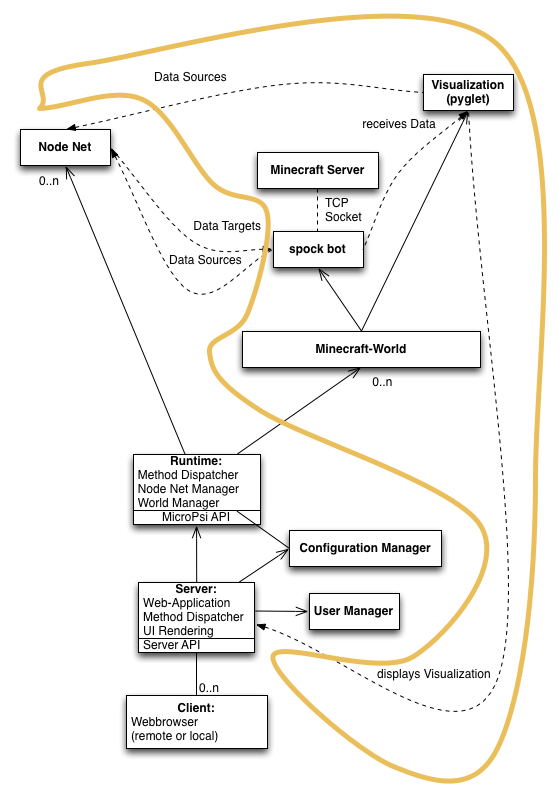
\includegraphics[width=10cm]{graphics/UML_MicroPsi_mit_spock_und_rahmen}
  \caption{The new architecture of MicroPsi with the Minecraft interface. New modules are framed orange.}
  \label{uml_mc}
\end{figure}

The \texttt{minecraftVisualisation} module can be exchanged or cut off completely very easily, as no other modules depend on it. Instead of the visualisation, a placeholder image can be displayed in the web interface, which does not effect the functionality of the simulation. The \texttt{minecraftVisualisation} module itself depends on the data structures of the \texttt{minecraftClient}, though. This means, exchanging the \texttt{minecraftClient} would require adjustments of the \texttt{minecraftVisualisation}, to still function as intended. The same holds true for the \emph{data sources} and \emph{targets} in the \texttt{minecraftWorld}.

    \section{Using \texttt{Spock} as the \texttt{minecraftClient}}

As mentioned above, the purpose of the \texttt{minecraftClient} is to manage the communication with the Minecraft server and to provide a representation of the agent's environment.

The calculation of the simulation environment, does not take place in MicroPsi itself, but on a regular Minecraft Server. Instead, \texttt{Spock} is integrated into MicroPsi and represents the simulation world towards it. \texttt{Spock} (in the following the \texttt{minecraftClient}) communicates with the Minecraft server via the client server protocol and provides data that can be used as \emph{data sources} for the world adapter and translates the data from the \emph{data targets} to actions in the simulation environment. That way, to MicroPsi it looks like the \texttt{minecraftClient} is the simulation environment itself, where, in fact, it is the interface to the game world server.

The original event loop of the bot framework had to be dissolved and rebuilt as an \texttt{advanceClient} function that is called as a part of the world adapter's step function. The event-loop and -handling of the \texttt{minecraftClient} had to be slightly modified to work with MicroPsi. It should be noted that the frequency, with which the framework steps the bot, has to be at least chosen high enough (about 10/s), so that Spock is able to regularly send the necessary keep-alive-signals, to not get kicked from the server.

For every iteration of the event loop, the \texttt{minecraftClient} reads incoming data from the socket, dispatches the read packages appropriately and eventually checks the MicroPsi \emph{data targets} to perform an action---if necessary~(see figure~\ref{spock_loop}). Note that the described event loop of the original \texttt{Spock} is not a loop anymore, but each iteration is invoked as a part of the world adapters step function.


\begin{wrapfigure}{r}{0.4\textwidth}
  \begin{center}
    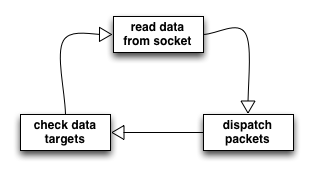
\includegraphics[width=0.4\textwidth]{graphics/spock_eventloop}
  \end{center}
  \caption{The \texttt{minecraftClient}'s event loop}
  \label{spock_loop}
\end{wrapfigure}

Eventually, useful data sources had to be picked and a system of data targets and their translation to actions had to be implemented. In most cases, performing actions means to let Spock send a particular set of packets to the Minecraft server.

        \subsection{Overview of the minecraftClient}
The \texttt{minecraftClient} is heavily based on \texttt{Spock}, that has been developed as an educational project. The scope of this project was to build a pure Python Minecraft bot framework without dependencies. This has been achieved with one minor exception: if one would like to connect the bot to an official Minecraft online server, the packets have to be encrypted using the Python cryptography library PyCrypto.

The \texttt{minecraftClient} runs as a part of the world runner thread. It consists of several classes. 

The main class, \texttt{minecraftClient}, holds references to instances of the classes BoundBuffer,  World and Packet. Furthermore, basic data structures are stored in the files cflags and mcdata.

The class \texttt{BoundBuffer} is an implementation of a buffer that matches the particular needs of sending and receiving Minecraft packets.

The class \texttt{World} holds the internal representation of the gameworld. It brings functions, data structures and subclasses to represent chunks and to obtain information about which block sits where. In its heart, it manages a dictionary, that stores chunks as binary data.

The class \texttt{Packet} represents a Minecraft packet and brings functions to encode and decode it (being read from a BoundBuffer) to get to its payload or to be able to send it to the Server.

The file \texttt{packet\_handlers.py} provides a class for each packet that the client is supposed to deal with by default. The following listing gives an example.


		\begin{figure}[ht]
			\centering
			\begin{minipage}{11cm}
				\begin{pseudocode}
#Chunk Data - Update client World state
@phandle(0x33)
class handle33(BaseHandle):
	@classmethod
	def ToClient(self, client, packet):
		client.world.unpack_column(packet)
					\end{pseudocode}
				\caption{Handling a Chunk Data packet}
				\label{packet_handling}
			\end{minipage}
		\end{figure}

The dictionary \texttt{cflags} provides the Socket codes.
The file \texttt{mcdata.py} provides dictionaries for the datatypes, block type codes, packet names and structures of packets of the Minecraft protocol.

In the file \texttt{nbt.py} several classes for dealing with the NBT file format exist.

The file \texttt{timer.py} contains the classes \texttt{EventTimer}, \texttt{TickTimer} and \texttt{ThreadedTimer}, which provide measures for the timing of the Minecraft world.

The client sets up a socket to the server, starts of with a handshake to from then on facilitate packet based communication with the server.

        \subsection{Extensions to the \texttt{minecraftClient}}
It was aimed for to extend the original client in a way that it would fit in nicely as a simulation world for MicroPsi.
        
A reference to the new class \texttt{PsiDispatcher} has been added to the \texttt{minecraftClient}. Its purpose is to check the \texttt{minecraftWorld}'s data targets frequently and invoke appropriate actions, if necessary. The following figure provides a simplified example of the resulting architecture. The \texttt{PsiDispatcher} is called as a part of the \texttt{advanceClient} function. It checks each available data target, and if necessary invokes an appropriate action (eg. sending a packet). Listing \ref{listing_dispatch} is an example for the data targets that indicates that the agent is supposed to move one block towards the direction of the x-axis. %TODO show simplified example

		\begin{figure}[ht]
			\centering
			\begin{minipage}{11cm}
				\begin{pseudocode}
#check for MicroPsi input
if self.client.move_x > 0:
    self.client.push(Packet(ident = 0x0B, data = {
        'x': (self.client.position['x'] - 1) / 1,
        'y': self.client.position['y'] / 1,
        'z': self.client.position['z'] / 1,
        'on_ground': False,
        'stance': self.client.position['y'] + 0.11
        }))
					\end{pseudocode}
				\caption{Dispatching the events regarding to the move-x data target}
				\label{listing_dispatch}
			\end{minipage}
		\end{figure}

The event loop has been replaced by the function \texttt{advanceClient} that is called for every simulation step. For example, one iteration could mean receiving and storing new block data from the Minecraft Server, sending default responses to the received packets, checking the MicroPsi data targets for moving and if necessary send a "Player Position" packet to the Minecraft server.

\begin{figure}[h]
  \centering
    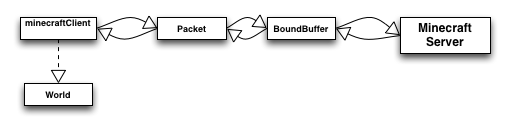
\includegraphics[width=10cm]{graphics/spock_overview}
  \caption{An overview of the most import classes of the \texttt{minecraftClient} in respect to the communication with a Minecraft Server}
  \label{spock_overview}
\end{figure}

    \section{Module \texttt{minecraftVisualisation}}
That being said, the other important part of this project is the visualisation component. It contains classes that provide an interface to the OpenGL context that is the visualisation. This section gives an overview about what data sources the visualisation uses and how it could be replaced or extended. Inside the \texttt{minecraftWorld}'s step function, the visualisation module is called to generate a 3D model of the Minecraft world and the agent within. There are two main reasons for this. The first reason is that the agent's behaviour within the simulation environment is supposed to be visually monitored from the MicroPsi web interface---in a both efficient and pleasurable manner. The second reason is that the image data is supposed to be processed by the node net as a data source itself in the future.

The visualisation component reads from the \texttt{minecraftClient}'s internal gameworld representation to generate the 3D model. This means that, from pure Minecraft world data, a 3D-visualisation has to be generated from within the MicroPsi Python code. It should contain a perspective that gives a good overview over the bots environment and forward it to the web interface. The visualisation is in it's core based on ``Minecraft'' by Michael Fogleman.

Specifically, the representation of the chunk, the agent is located in, is fetched and for each solid cube in this chunk, a corresponding cube is rendered within the visualisation using Pyglet's OpenGL abstraction~(see figure~\ref{vis_screen}). Each block gets textures according to its type. The implemented format for the textures is compatible to the widely available Minecraft texture packs. That way, the visualisation's look can be changed completely within seconds. The resulting images are exported as JPEG files. Then, they are displayed in the web interface. A refresh rate of six or more images per second creates the impression of a video stream.

The module \texttt{minecraftVisualisation} consists of two classes. The class \texttt{Window} inherits from \texttt{pyglet.window.Window} and therefore initialises the OpenGL context. For every call of the \texttt{advanceVisualisation} function, it updates the 3D model according to the world representation inside the minecraftClient and renders it. A PNG snapshot of the frame buffer is generated and displayed in the web interface.

The class \texttt{Model} is also used as a part of the \texttt{advanceVisualisation} function. It contains functions for adding and removing blocks from the OpenGL canvas. The textures for the blocks are loaded from PNG images, stored as \texttt{pyglet.graphics.TextureGroups} and are assigned to vertices when needed.



\begin{figure}[h]
  \centering
    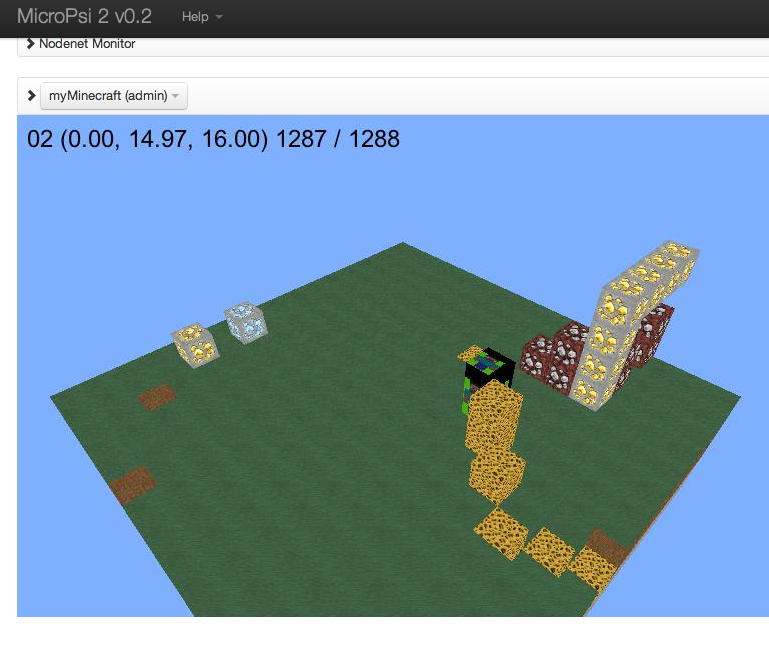
\includegraphics[width=10cm]{graphics/visualisation_screen}
  \caption{An Image generated by the visualisation component}
  \label{vis_screen}
\end{figure}



Similar to \texttt{Spock}, \texttt{Minecraft} by Michael Fogleman implements it's own event-loop and -handling. Again, the event loop had to be disassembled and rebuilt as a part of the world adapter's step function, which advances the visualisation with every step.

    \section{Module \texttt{minecraftWorld}}
The world adapter contains two classes. The class \texttt{MinecraftWorld} inherits from the MicroPsi class \texttt{world} and provides the assets for the web interface, an \texttt{init} function and the \texttt{step} function. The class \texttt{Braitencraft} holds of the actual world adapter. In it, the \emph{data sources} and \emph{targets} are defined as dictionaries and an update function advances the life of the client.
    
\paragraph{Data Targets and sources}$\;$ \\

As a proof of concept, four data sources have been defined, that symbolize sensors, that detect, if a block of diamond in the current section is either before, behind, left or right of the client. The data targets are filled, as it is outlined in figure~\ref{listing_sensors}.

On the other hand, data targets have been defined, that represent actuators for moving forwards, backwards, left and right.

    \section{Case Study}
To explain the usage of this implementation, an example is given in the following. An agent is placed in a Minecraft world. It shall contain the four previously mentioned sensors that point to the positive and negative x- and y-axes. Theses sensors detect if a diamond ore block has been placed in the current chunk, in the direction they are facing. The agent furthermore consists of four actuators that make the agent move towards each of the same four directions. Next, the sensors get connected to the corresponding actuators, which will lead to an agent being attracted towards a placed diamond block.

To conclude the experiment, a chunk in a Minecraft world is set up that way, that it contains only a plane, without other obstacles, that the agent might move around on freely, as well as a diamond block that is placed at its center. 

Then, the agent is placed in one of the chunk`s corners. We furthermore define that the activation of the sensors equals the distance to the diamond block in the regarding direction. The data sources get filled through searching in the entire section, as figure~\ref{listing_sensors} displays.

		\begin{figure}[ht]
			\centering
			\begin{minipage}{18cm}
				\begin{pseudocode}
for y in range(0, 16):
 current_section = ent_column.chunks[int((bot_block[1] + y -  2) / 16)]
 if current_section != None:
  for x in range(0, 16):
   for z in range(0, 16):
    current_block = current_section['block_data'].get(x, _block[1] + y - 10 / 2) \% 16), z)
    if current_block == 56: #Diamond Ore
     diamond_coords = (x + x_chunk * 16,y,z + z_chunk * 16)
      self.datasources['diamond_offset_x'] = bot_block[0] - coords[0] - 3
      self.datasources['diamond_offset_z'] = bot_block[2] - coords[2] - 3
      self.datasources['diamond_offset_x_'] = ((bot_block[0] - coords[0]) * -1) - 3
      self.datasources['diamond_offset_z_'] = ((bot_block[2] - coords[2]) * -1) - 3
			\end{pseudocode}
		\caption{Searching for a diamond block an filling the data sources with the distance towards it}
		\label{listing_sensors}
	\end{minipage}
\end{figure}
    
In every step of the world, the client will check the data targets and therefore move towards the diamond. Once it gets to a distance towards the diamond, that is below a defined threshold, the sensors will stop sending activation, and the agent will stop moving towards it. Note that if the node net runner and the world runner run asynchronously, there might be a delay in the shift of behaviour of the agent. Hence, it is advised, to run them synchronously or at least with a timing close to each other.

In the node net editor, we set up the corresponding node net, as it can be seen in figure~\ref{nodenet_setup}. Now, the world writes the activation from the sensors to the actuators in every iteration of the step function.

\begin{figure}[h]
  \centering
    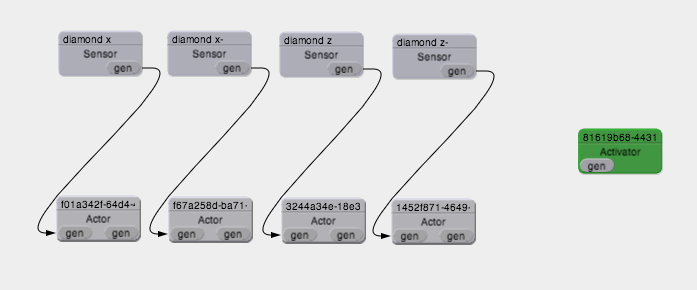
\includegraphics[width=10cm]{graphics/nodenet_setup}
  \caption{A node net setup for a Diamond-finding experiment}
  \label{nodenet_setup}
\end{figure}

If we start a simulation like this, the nodes of the sensors that point to the diamond light up green and their activation is forwarded to the actuators. The bot moves towards the diamond until it is closer than the sensor's threshold, to not detect the diamond anymore---for this experiment the threshold has been set to two blocks. Then it stops moving~(see figure \ref{diamond_screens}).

\begin{figure}[h]
  \centering
    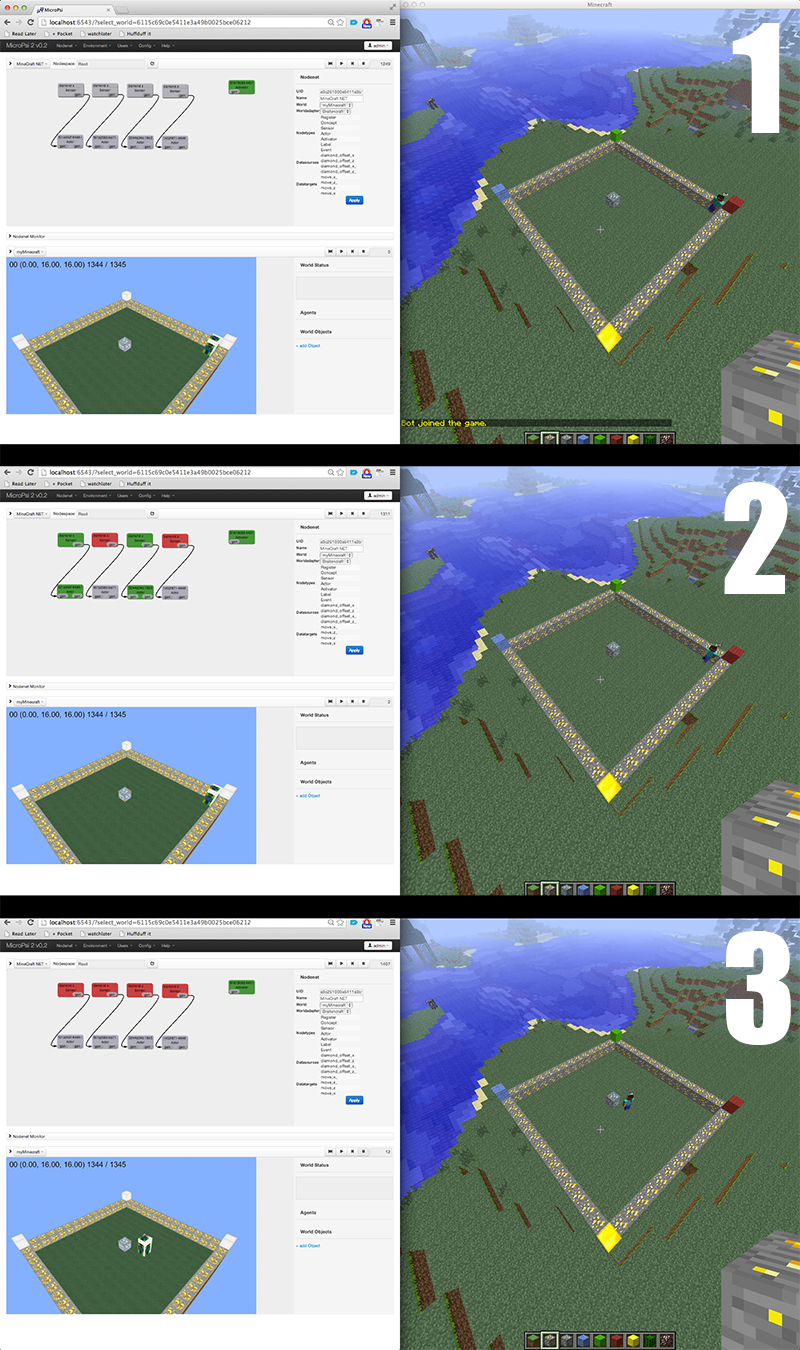
\includegraphics[width=10cm]{graphics/diamond_screens}
  \caption{1. Neither node net, nor agent show any activivity, as the experiment did not start yet.  2. The sensors that indicate a diamond towards the negative x- and z-axes light up green---so do the according actuators. The agent starts moving.  3. The agent arrived close enough to the diamond, that the sensors stop forwarding activation. The agent stops moving.}
  \label{diamond_screens}
\end{figure}

        \subsection{Evaluation}
Now, that a proof-of-concept experiment has been concluded, the implementation can be evaluated.
The experiment obviously shows that an interface in between a Minecraft world and the MicroPsi framework has been implemented. In the experiment, the agent concludes the appropriate action, if a node net actuator node receives activation and stops doing so, when it stops receiving activation.

With MicroPsi node nets in the back, more complex experiments can now be thought of and implemented, that lead to more complex behaviours of the agent.

An issue that remains concerning is that the reaction time in between changes in the node net and the according changes of the agent's behaviour seems to be too long, for differing timing of the node net runner and the world runner.

This issue could be resolved, by making the bot faster---for example, by sending the visualisation image data directly to the web interface, without writing it to the hard disk first.

    \section{Summary}
This chapter presented the implementation of the Minecraft interface for MicroPsi, which consists of the modules \texttt{minecraftClient}, \texttt{minecraftVisualisation} and \texttt{minecraftWorld}. The \texttt{minecraftClient} facilitates the communication with the Minecraft server; the \texttt{minecraftVisualisation} delivers OpenGL rendered image data of the environment and the \texttt{minecraftWorld} serves as the actual world adapter in between the \texttt{minecraftClient} and MicroPsi.
Next, a case study has been performed and evaluated. A MicroPsi client had to move towards a block of a particular type. It showed that the interface is functional and ready for more sophisticated experiments.
With the implementation of the interface and the following proof-of-concept case study the scope of this thesis has been completed. The last chapter contains a summary and an outlook towards future applications.